%\documentclass[handout]{beamer} % \pause disabled
\documentclass[t]{beamer} % \pause enabled
%%%%%%%%%%%%%%%%% Arya's
\usepackage{color,hyperref}
\hypersetup{colorlinks,breaklinks,linkcolor=darkblue,urlcolor=darkblue, anchorcolor=darkblue,citecolor=darkblue}
\usepackage{amssymb,amsmath,amsthm,amsfonts}
\usepackage{mathtools}
\usepackage{enumerate}
\definecolor{darkgreen}{rgb}{0,0.55,0}
\definecolor{orange}{rgb}{1,0.55,0}
\definecolor{darkblue}{rgb}{0.0,0.0,0.5}
\def\Arya#1{{\textcolor{darkgreen}{Arya note: #1}}}
\def\emphr#1{{\textcolor{red}{#1}}}
\def\emphg#1{{\textcolor{darkgreen}{#1}}}
\def\emphb#1{{\textcolor{darkblue}{#1}}}
\usepackage{pifont}
\newcommand{\cmark}{\ding{51}}%
\newcommand{\xmark}{\ding{55}}%
\usepackage{bbm}
\def\datadm{data from a study of \dmel adaptation to alternating temperatures}
\def\comale{\text{{\sc Clear}}}
\newcommand{\dataset}{{\cal D}}
\newcommand{\fracpartial}[2]{\frac{\partial #1}{\partial  #2}}
\newcommand{\phibp}{\phi_{ \hspace{-0.025in}\scalebox{.45}{\text{ BP}}}}
\newcommand{\phics}{\phi_{ \hspace{-0.025in}\scalebox{.45}{\text{ CS}}}}
\newcommand{\lone}{$\ell_1$-norm }
%\def\lll{\mbox{\ell_1}}
\def\dmel{\emph{D. melanogaster }}

\DeclareMathOperator{\tw}{tw}
\DeclareMathOperator{\local}{local}
\DeclareMathOperator{\range}{range}
\DeclareMathOperator{\Path}{Path}
\DeclareMathOperator{\Sg}{Sg}
\DeclareMathOperator{\spt}{SP}
\DeclareMathOperator{\avg}{avg}
\DeclareMathOperator{\nbd}{\mathcal{N}}
\DeclareMathOperator{\parent}{Pa}
\DeclareMathOperator{\Cq}{Cq}
\DeclareMathOperator{\TW}{TW}
\DeclareMathOperator{\approxML}{ApproxML}
\DeclareMathOperator{\Bethe}{Bethe}
\DeclareMathOperator{\TRW}{TRW}
\DeclareMathOperator{\conv}{Conv}
\DeclareMathOperator{\dir}{Dir}
\DeclareMathOperator{\mult}{Mult}
\DeclareMathOperator{\cat}{Cat}
\DeclareMathOperator{\crp}{CRP(\gamma)}
\DeclareMathOperator{\ncrp}{nCRP}
\DeclareMathOperator{\node}{node}
\DeclareMathOperator{\nodes}{nodes}
\DeclareMathOperator{\pr}{Pr}
\DeclareMathOperator{\dom}{\bf Dom}
\DeclareMathOperator{\lbp}{LBP}
\DeclareMathOperator{\Corr}{Corr}
\DeclareMathOperator{\hCorr}{\widehat{Corr}}
\DeclareMathOperator{\hSc}{\widehat{\mathcal{S}}}
\DeclareMathOperator{\tr}{Tr}
\DeclareMathOperator{\mst}{MST}
\DeclareMathOperator{\supp}{Supp}
\DeclareMathOperator{\dtv}{d_{TV}}
\DeclareMathOperator{\hdtv}{\hd_{TV}}
\DeclareMathOperator*{\argmin}{arg\,min}
\DeclareMathOperator*{\argmax}{arg\,max}
\DeclareMathOperator*{\esssup}{ess\,sup}
\DeclareMathOperator*{\essinf}{ess\,inf}
\DeclareMathOperator{\dist}{dist}
\DeclareMathOperator{\rank}{Rank}
\DeclareMathOperator{\Krank}{Rank_K}
\DeclareMathOperator{\Det}{Det}
\DeclareMathOperator{\poiss}{Poiss}
\DeclareMathOperator{\unif}{Unif} \DeclareMathOperator{\Deg}{Deg}
\def\simiid{{\overset{i.i.d.}{\sim}}}
\def\lcv{{\,\,\underset{cv}{\leq}\,\,}}
\def\gcv{{\,\,\underset{cv}{\geq}\,\,}}
\def\lcx{{\,\,\underset{cx}{\leq}\,\,}}
\def\gcx{{\,\,\underset{cx}{\geq}\,\,}}
\def\leqst{{\,\,\overset{st}{\leq}\,\,}}
\def\geqst{{\,\,\overset{st}{\geq}\,\,}}
\def\eqdist{{\,\,\overset{d}{=}\,\,}}
\def\geqrh{{\,\,\overset{rh}{\geq}\,\,}}
\def\geqlr{{\,\,\overset{lr}{\geq}\,\,}}
\def\eqlr{{\,\,\overset{lr}{=}\,\,}}
\def\tha{{\mbox{\tiny th}}}

\DeclareMathOperator{\Aug}{Aug}
\DeclareMathOperator{\watts}{Watts}
\DeclareMathOperator{\girth}{Girth}
\DeclareMathOperator{\PL}{PL}
\DeclareMathOperator{\LP}{LP}
\DeclareMathOperator{\ER}{ER}
\DeclareMathOperator{\reg}{Reg}
\DeclareMathOperator{\Var}{Var}
\DeclareMathOperator{\hSigma}{\widehat{\Sigma}}
\DeclareMathOperator{\Cov}{Cov}
\DeclareMathOperator{\Poiss}{Poiss}
\DeclareMathOperator{\Diag}{Diag}
\DeclareMathOperator{\Diam}{Diam}
\def\erf{\mbox{erf}}
\def\erfc{\mbox{erfc}}
\def\qfunc{\mbox{Q}}
%\def\myexp{\mbox{e}}
\def\snr{\mbox{{SNR}}}
\def\signum{\mbox{sgn}}
\def\Card{\mbox{Card}}
\DeclareMathOperator*{\plim}{plim}
\def\convd{\overset{d}\rightarrow}
\def\convp{\overset{p}\rightarrow}
\newcommand\indep{\protect\mathpalette{\protect\independenT}{\perp}}
\def\independenT#1#2{\mathrel{\rlap{$#1#2$}\mkern2mu{#1#2}}}
\def\pl{{\parallel}}
\DeclarePairedDelimiter\norm{\lVert}{\rVert}
\DeclarePairedDelimiter\nuclearnorm{\lVert}{\rVert_*}
\DeclarePairedDelimiter\onenorm{\lVert}{\rVert_1}
\DeclarePairedDelimiter\znorm{\lVert}{\rVert_0}
\def\rinfnorm{\rVert_{\infty}}
\DeclarePairedDelimiter\infnorm{\lVert}{\rinfnorm}
\def\lnorm{{\lvert\!\lvert\!\lvert}}
\def\rnorm{{\rvert\!\rvert\!\rvert}}
\DeclarePairedDelimiter\gennorm{\lnorm}{\rnorm}
 \DeclarePairedDelimiter\abs{\lvert}{\rvert}
 \DeclarePairedDelimiter\geninfnorm{\lnorm}{\rnorm_{\infty}}
 \DeclarePairedDelimiter\genonenorm{\lnorm}{\rnorm_{1}}
\DeclareMathOperator{\atanh}{atanh}
 \DeclareMathOperator{\sech}{sech}
 \def\0{{\bf 0}}

\DeclareMathOperator{\lea}{\overset{(a)}{\leq}}
\DeclareMathOperator{\leb}{\overset{(b)}{\leq}}
\DeclareMathOperator{\lec}{\overset{(c)}{\leq}}
\DeclareMathOperator{\led}{\overset{(d)}{\leq}}
\DeclareMathOperator{\lee}{\overset{(e)}{\leq}}

\DeclareMathOperator{\eqa}{\overset{(a)}{=}}
\DeclareMathOperator{\eqb}{\overset{(b)}{=}}
\DeclareMathOperator{\eqc}{\overset{(c)}{=}}
\DeclareMathOperator{\eqd}{\overset{(d)}{=}}
\DeclareMathOperator{\eqe}{\overset{(e)}{=}}

\DeclareMathOperator{\gea}{\overset{(a)}{\geq}}
\DeclareMathOperator{\geb}{\overset{(b)}{\geq}}
\DeclareMathOperator{\gec}{\overset{(c)}{\geq}}
\DeclareMathOperator{\ged}{\overset{(d)}{\geq}}
\DeclareMathOperator{\gee}{\overset{(e)}{\geq}}

\def\viz{{viz.,\ \/}}
\def\ie{{i.e.,\ \/}}
\def\eg{{e.g.,\ \/}}
\def\etc{{etc.  }}
\def\ifff{{iff  }}
\def\as{{a.s.  }}
\def\st{{s.t.  }}
\def\wpone{{w.p.}\,1\,\,}
\def\wpp{{w.p.p.}\,\,}
\def\for{\,\,\mbox{for}\quad}
\def\ifmbox{\,\,\mbox{if}\quad}
\def\nn{\nonumber}
%\def\qed{\hfill$\Box$}

\def\qed{\hfill\hbox{${\vcenter{\vbox{
    \hrule height 0.4pt\hbox{\vrule width 0.4pt height 6pt
    \kern5pt\vrule width 0.4pt}\hrule height 0.4pt}}}$}}
\def\complx{\mathbb{C}}

%%%%%%%%%%%%%%%%%%%%%%%%%%%%%%%%%%%%%%%%%%%%%%%%%%%%%%%%%%%%% Color

\def\tcr{\textcolor{red}}
\def\tcb{\textcolor{blue}}
\def\tcg{\textcolor{green}}
\def\tcw{\textcolor{white}}
\def\tcm{\textcolor{magenta}}
\def\tccyan{\textcolor{cyan}}
\def\tcv{\textcolor{violet}}
\definecolor{myred}{rgb}{0.3,0.0,0.7}
\definecolor{dkg}{rgb}{0.1,0.7,0.2}
\definecolor{dkb}{rgb}{0.0,0.2,0.8}

\def\tcdkb{\textcolor{dkb}}
\def\tcdkg{\textcolor{dkg}}


%%%%%%%%%%%%%%%%%%%%%%%%%%%%%%%%%%%%%%%%%%%%%%%%%%%%%%%%%%%%%
\newcommand{\Amsc}{\mathscr{A}}
\newcommand{\Cmsc}{\mathscr{C}}
\newcommand{\Dmsc}{\mathscr{D}}
\newcommand{\Emsc}{\mathscr{E}}
\newcommand{\Fmsc}{\mathscr{F}}
\newcommand{\Gmsc}{\mathscr{G}}
\newcommand{\Hmsc}{\mathscr{H}}
\newcommand{\Kmsc}{\mathscr{K}}
\newcommand{\Nmsc}{\mathscr{N}}
\newcommand{\Pmsc}{\mathscr{P}}
\newcommand{\Qmsc}{\mathscr{Q}}
\newcommand{\Rmsc}{\mathscr{R}}
\newcommand{\Smsc}{\mathscr{S}}
\newcommand{\Tmsc}{\mathscr{T}}
\newcommand{\Umsc}{\mathscr{U}}
\newcommand{\Xmsc}{\mathscr{X}}
\newcommand{\Ymsc}{\mathscr{Y}}

%%%%%%%%%%%%%%%%%%%%%%%%%%%%%%%%%%%%%%%%%%%%%%%%%%%%%%%%%%%%% Hat
\def\ha{\widehat{a}}
\def\hb{\widehat{b}}
\def\hc{\widehat{c}}
\def\hd{\widehat{d}}
\def\he{\widehat{e}}
\def\hf{\widehat{f}}
\def\hg{\widehat{g}}
\def\hh{\widehat{h}}
\def\hi{\widehat{i}}
\def\hj{\widehat{j}}
\def\hk{\widehat{k}}
\def\hl{\widehat{l}}
\def\hm{\widehat{m}}
\def\hn{\widehat{n}}
\def\ho{\widehat{o}}
\def\hp{\widehat{p}}
\def\hq{\widehat{q}}
\def\hr{\widehat{r}}
\def\hs{\widehat{s}}
\def\hatt{\widehat{t}}
\def\hu{\widehat{u}}
\def\hv{\widehat{v}}
\def\hw{\widehat{w}}
\def\hx{\widehat{x}}
\def\hy{\widehat{y}}
\def\hz{\widehat{z}}

\def\hA{\widehat{A}}
\def\hB{\widehat{B}}
\def\hC{\widehat{C}}
\def\hD{\widehat{D}}
\def\hE{\widehat{E}}
\def\hF{\widehat{F}}
\def\hG{\widehat{G}}
\def\hH{\widehat{H}}
\def\hI{\widehat{I}}
\def\hJ{\widehat{J}}
\def\hK{\widehat{K}}
\def\hL{\widehat{L}}
\def\hM{\widehat{M}}
\def\hN{\widehat{N}}
\def\hO{\widehat{O}}
\def\hP{\widehat{P}}
\def\hQ{\widehat{Q}}
\def\hR{\widehat{R}}
\def\hS{\widehat{S}}
\def\hT{\widehat{T}}
\def\hU{\widehat{U}}
\def\hV{\widehat{V}}
\def\hW{\widehat{W}}
\def\hX{\widehat{X}}
\def\hY{\widehat{Y}}
\def\hZ{\widehat{Z}}
\def\hlambda{\widehat{\lambda}}
\def\hpi{\widehat{\pi}}
\def\hnu{\widehat{\nu}}
\def\hbd{\widehat{\mathbf{d}}}
\def\bLambda{\mathbf{\Lambda}}


%%%%%%%%%%%%%%%%%%%%%%%%%%%%%%%%%%%%%%%%%%%%%%%%%%%%%%%%%%%%% Vector
\def\valpha{\vec{\alpha}}
\def\va{\vec{a}}
\def\vb{\vec{b}}
\def\vc{\vec{c}}
\def\vd{\vec{d}}
\def\ve{\vec{e}}
\def\vf{\vec{f}}
\def\vg{\vec{g}}
\def\vh{\vec{h}}
\def\vi{\vec{i}}
\def\vj{\vec{j}}
\def\vk{\vec{k}}
\def\vl{\vec{l}}
\def\vm{\vec{m}}
\def\vn{\vec{n}}
\def\vo{\vec{o}}
\def\vp{\vec{p}}
\def\vq{\vec{q}}
\def\vr{\vec{r}}
\def\vs{\vec{s}}
\def\vt{\vec{t}}
\def\vu{\vec{u}}
\def\vv{\vec{v}}
\def\vw{\vec{w}}
\def\vx{\vec{x}}
\def\vy{\vec{y}}
\def\vz{\vec{z}}

\def\vA{\vec{A}}
\def\vB{\vec{B}}
\def\vC{\vec{C}}
\def\vD{\vec{D}}
\def\vE{\vec{E}}
\def\vF{\vec{F}}
\def\vG{\vec{G}}
\def\vH{\vec{H}}
\def\vI{\vec{I}}
\def\vJ{\vec{J}}
\def\vK{\vec{K}}
\def\vL{\vec{L}}
\def\vM{\vec{M}}
\def\vN{\vec{N}}
\def\vO{\vec{O}}
\def\vP{\vec{P}}
\def\vQ{\vec{Q}}
\def\vR{\vec{R}}
\def\vS{\vec{S}}
\def\vT{\vec{T}}
\def\vU{\vec{U}}
\def\vV{\vec{V}}
\def\vW{\vec{W}}
\def\vX{\vec{X}}
\def\vY{\vec{Y}}
\def\vZ{\vec{Z}}

%%%%%%%%%%%%%%%%%%%%%%%%%%%%%%%%%%%%%%%%%%%%%%%%%%%%%%%%%%%%% Bold
\def\bfalpha{{\boldsymbol {\alpha}}}
\def\bfnu{{\boldsymbol {\nu}}}
\def\bfeta{{\boldsymbol {\eta}}}
\def\bfzero{{\mathbf{0}}}
\def\bfone{{\mathbf{1}}}
\def\bfa{{\mathbf a}}
\def\bfb{{\mathbf b}}
\def\bfc{{\mathbf c}}
\def\bfd{{\mathbf d}}
\def\bfe{{\mathbf e}}
\def\bff{{\mathbf f}}
\def\bfg{{\mathbf g}}
\def\bfh{{\mathbf h}}
\def\bfi{{\mathbf i}}
\def\bfj{{\mathbf j}}
\def\bfk{{\mathbf k}}
\def\bfl{{\mathbf l}}
\def\bfm{{\mathbf m}}
\def\bfn{{\mathbf n}}
\def\bfo{{\mathbf o}}
\def\bfp{{\mathbf p}}
\def\bfq{{\mathbf q}}
\def\bfr{{\mathbf r}}
\def\bfs{{\mathbf s}}
\def\bft{{\mathbf t}}
\def\bfu{{\mathbf u}}
\def\bfv{{\mathbf v}}
\def\bfw{{\mathbf w}}
\def\bfx{{\mathbf x}}
\def\bfy{{\mathbf y}}
\def\bfz{{\mathbf z}}

\def\bfA{{\mathbf A}}
\def\bfB{{\mathbf B}}
\def\bfC{{\mathbf C}}
\def\bfD{{\mathbf D}}
\def\bfE{{\mathbf E}}
\def\bfF{{\mathbf F}}
\def\bfG{{\mathbf G}}
\def\bfH{{\mathbf H}}
\def\bfI{{\mathbf I}}
\def\bfJ{{\mathbf J}}
\def\bfK{{\mathbf K}}
\def\bfL{{\mathbf L}}
\def\bfM{{\mathbf M}}
\def\bfN{{\mathbf N}}
\def\bfO{{\mathbf O}}
\def\bfP{{\mathbf P}}
\def\bfQ{{\mathbf Q}}
\def\bfR{{\mathbf R}}
\def\bfS{{\mathbf S}}
\def\bfT{{\mathbf T}}
\def\bfU{{\mathbf U}}
\def\bfV{{\mathbf V}}
\def\bfW{{\mathbf W}}
\def\bfX{{\mathbf X}}
\def\bfY{{\mathbf Y}}
\def\bfZ{{\mathbf Z}}


%%%%%%%%%%%%%%%%%%%%%%%%%%%%%%%%%%%%%%%%%%%%%%%%%%%%%%%%%%%%% Bold Symbols
\def\alphabf{\hbox{\boldmath$\alpha$\unboldmath}}
\def\betabf{\hbox{\boldmath$\beta$\unboldmath}}
\def\gammabf{\hbox{\boldmath$\gamma$\unboldmath}}
\def\deltabf{\hbox{\boldmath$\delta$\unboldmath}}
\def\epsilonbf{\hbox{\boldmath$\epsilon$\unboldmath}}
\def\zetabf{\hbox{\boldmath$\zeta$\unboldmath}}
\def\etabf{\hbox{\boldmath$\eta$\unboldmath}}
\def\iotabf{\hbox{\boldmath$\iota$\unboldmath}}
\def\kappabf{\hbox{\boldmath$\kappa$\unboldmath}}
\def\lambdabf{\hbox{\boldmath$\lambda$\unboldmath}}
\def\mubf{\hbox{\boldmath$\mu$\unboldmath}}
\def\nubf{\hbox{\boldmath$\nu$\unboldmath}}
\def\xibf{\hbox{\boldmath$\xi$\unboldmath}}
\def\pibf{\hbox{\boldmath$\pi$\unboldmath}}
\def\rhobf{\hbox{\boldmath$\rho$\unboldmath}}
\def\sigmabf{\hbox{\boldmath$\sigma$\unboldmath}}
\def\taubf{\hbox{\boldmath$\tau$\unboldmath}}
\def\upsilonbf{\hbox{\boldmath$\upsilon$\unboldmath}}
\def\phibf{\hbox{\boldmath$\phi$\unboldmath}}
\def\chibf{\hbox{\boldmath$\chi$\unboldmath}}
\def\psibf{\hbox{\boldmath$\psi$\unboldmath}}
\def\omegabf{\hbox{\boldmath$\omega$\unboldmath}}
\def\inftybf{\hbox{\boldmath$\infty$\unboldmath}}
\def\hSigmabf{\hbox{$\widehat{\bf \Sigma}$}}
\def\Sigmabf{\hbox{$\bf \Sigma$}}
\def\Upsilonbf{\hbox{$\bf \Upsilon$}}
\def\Omegabf{\hbox{$\bf \Omega$}}
\def\Deltabf{\hbox{$\bf \Delta$}}
\def\Gammabf{\hbox{$\bf \Gamma$}}
\def\Thetabf{\hbox{$\bf \Theta$}}
\def\Lambdabf{\mbox{$ \bf \Lambda $}}
\def\Xibf{\hbox{\bf$\Xi$}}
\def\Pibf{{\bf \Pi}}
\def\thetabf{{\mbox{\boldmath$\theta$\unboldmath}}}
\def\Upsilonbf{\hbox{\boldmath$\Upsilon$\unboldmath}}
\newcommand{\Phibf}{\mbox{${\bf \Phi}$}}
\newcommand{\Psibf}{\mbox{${\bf \Psi}$}}
\def\olambda{\mathfrak{o}(\lambda)}
\def\complex{\mathfrak{C}}

%%%%%%%%%%%%%%%%%%%%%%%%%%%%%%%%%%%%%%%%%%%%%%%%%%%%%%%%%%%%% Bar
\def\brzero{{\overline{{0}}}}
\def\brone{{\overline{{1}}}}
\def\bra{{\overline{a}}}
\def\brb{{\overline{b}}}
\def\brc{{\overline{c}}}
\def\brd{{\overline{d}}}
\def\bre{{\overline{e}}}
\def\brf{{\overline{f}}}
\def\brg{{\overline{g}}}
\def\brh{{\overline{h}}}
\def\bri{{\overline{i}}}
\def\brj{{\overline{j}}}
\def\brk{{\overline{k}}}
\def\brl{{\overline{l}}}
\def\brm{{\overline{m}}}
\def\brn{{\overline{n}}}
\def\bro{{\overline{o}}}
\def\brp{{\overline{p}}}
\def\brq{{\overline{q}}}
\def\brr{{\overline{r}}}
\def\brs{{\overline{s}}}
\def\brt{{\overline{t}}}
\def\bru{{\overline{u}}}
\def\brv{{\overline{v}}}
\def\brw{{\overline{w}}}
\def\brx{{\overline{x}}}
\def\bry{{\overline{y}}}
\def\brz{{\overline{z}}}

\def\brA{{\overline{A}}}
\def\brB{{\overline{B}}}
\def\brC{{\overline{C}}}
\def\brD{{\overline{D}}}
\def\brE{{\overline{E}}}
\def\brF{{\overline{F}}}
\def\brG{{\overline{G}}}
\def\brH{{\overline{H}}}
\def\brI{{\overline{I}}}
\def\brJ{{\overline{J}}}
\def\brK{{\overline{K}}}
\def\brL{{\overline{L}}}
\def\brM{{\overline{M}}}
\def\brN{{\overline{N}}}
\def\brO{{\overline{O}}}
\def\brP{{\overline{P}}}
\def\brQ{{\overline{Q}}}
\def\brR{{\overline{R}}}
\def\brS{{\overline{S}}}
\def\brT{{\overline{T}}}
\def\brU{{\overline{U}}}
\def\brV{{\overline{V}}}
\def\brW{{\overline{W}}}
\def\brX{{\overline{X}}}
\def\brY{{\overline{Y}}}
\def\beZ{{\overline{Z}}}

%%%%%%%%%%%%%%%%%%%%%%%%%%%%%%%%%%%%%%%%%%%%%%%%%%%%%%%%%%%%% Bar Bold 
\def\bbfzero{{\overline{\mathbf{0}}}}
\def\bbfone{{\overline{\mathbf{1}}}}
\def\bbfa{{\overline{\mathbf a}}}
\def\bbfb{{\overline{\mathbf b}}}
\def\bbfc{{\overline{\mathbf c}}}
\def\bbfd{{\overline{\mathbf d}}}
\def\bbfe{{\overline{\mathbf e}}}
\def\bbff{{\overline{\mathbf f}}}
\def\bbfg{{\overline{\mathbf g}}}
\def\bbfh{{\overline{\mathbf h}}}
\def\bbfi{{\overline{\mathbf i}}}
\def\bbfj{{\overline{\mathbf j}}}
\def\bbfk{{\overline{\mathbf k}}}
\def\bbfl{{\overline{\mathbf l}}}
\def\bbfm{{\overline{\mathbf m}}}
\def\bbfn{{\overline{\mathbf n}}}
\def\bbfo{{\overline{\mathbf o}}}
\def\bbfp{{\overline{\mathbf p}}}
\def\bbfq{{\overline{\mathbf q}}}
\def\bbfr{{\overline{\mathbf r}}}
\def\bbfs{{\overline{\mathbf s}}}
\def\bbft{{\overline{\mathbf t}}}
\def\bbfu{{\overline{\mathbf u}}}
\def\bbfv{{\overline{\mathbf v}}}
\def\bbfw{{\overline{\mathbf w}}}
\def\bbfx{{\overline{\mathbf x}}}
\def\bbfy{{\overline{\mathbf y}}}
\def\bbfz{{\overline{\mathbf z}}}

\def\bbfA{{\overline{\mathbf A}}}
\def\bbfB{{\overline{\mathbf B}}}
\def\bbfC{{\overline{\mathbf{C}}}}
\def\bbfD{{\overline{\mathbf D}}}
\def\bbfE{{\overline{\mathbf E}}}
\def\bbfF{{\overline{\mathbf F}}}
\def\bbfG{{\overline{\mathbf G}}}
\def\bbfH{{\overline{\mathbf H}}}
\def\bbfI{{\overline{\mathbf I}}}
\def\bbfJ{{\overline{\mathbf J}}}
\def\bbfK{{\overline{\mathbf K}}}
\def\bbfL{{\overline{\mathbf L}}}
\def\bbfM{{\overline{\mathbf M}}}
\def\bbfN{{\overline{\mathbf N}}}
\def\bbfO{{\overline{\mathbf O}}}
\def\bbfP{{\overline{\mathbf P}}}
\def\bbfQ{{\overline{\mathbf Q}}}
\def\bbfR{{\overline{\mathbf R}}}
\def\bbfS{{\overline{\mathbf S}}}
\def\bbfT{{\overline{\mathbf T}}}
\def\bbfU{{\overline{\mathbf U}}}
\def\bbfV{{\overline{\mathbf V}}}
\def\bbfW{{\overline{\mathbf W}}}
\def\bbfX{{\overline{\mathbf X}}}
\def\bbfY{{\overline{\mathbf Y}}}
\def\bbfZ{{\overline{\mathbf Z}}}

%%%%%%%%%%%%%%%%%%%%%%%%%%%%%%%%%%%%%%%%%%%%%%%%%%%%%%%%%%%%% Calligraphic
\def\Ac{{\cal A}}
\def\Bc{{\cal B}}
\def\Cc{{\cal C}}
\def\Dc{{\cal D}}
\def\Ec{{\cal E}}
\def\Fc{{\cal F}}
\def\Gc{{\cal G}}
\def\Hc{{\cal H}}
\def\Ic{{\cal I}}
\def\Jc{{\cal J}}
\def\Kc{{\cal K}}
\def\Lc{{\cal L}}
\def\Mc{{\cal M}}
\def\Nc{{\cal N}}
\def\Oc{{\cal O}}
\def\Pc{{\cal P}}
\def\Qc{{\cal Q}}
\def\Rc{{\cal R}}
\def\Sc{{\cal S}}
\def\Tc{{\cal T}}
\def\Uc{{\cal U}}
\def\Vc{{\cal V}}
\def\Wc{{\cal W}}
\def\Xc{{\cal X}}
\def\Yc{{\cal Y}}
\def\Zc{{\cal Z}}


%%%%%%%%%%%%%%%%%%%%%%%%%%%%%%%%%%%%%%%%%%%%%%%%%%%%%%%%%%%%% Mathbb

\def\Abb{{\mathbb A}}
\def\BBb{{\mathbb B}}% different
\def\Cbb{{\mathbb C}}
\def\Dbb{{\mathbb D}}
\def\Ebb{{\mathbb E}}
\def\Fbb{{\mathbb F}}
\def\Gbb{{\mathbb G}}
\def\Hbb{{\mathbb H}}
\def\Ibb{{\mathbb I}}
\def\Jbb{{\mathbb J}}
\def\Kbb{{\mathbb K}}
\def\Lbb{{\mathbb L}}
\def\Mbb{{\mathbb M}}
\def\Nbb{{\mathbb N}}
\def\Obb{{\mathbb O}}
\def\Pbb{{\mathbb P}}
\def\Qbb{{\mathbb Q}}
\def\Rbb{{\mathbb R}}
\def\Sbb{{\mathbb S}}
\def\Tbb{{\mathbb T}}
\def\Ubb{{\mathbb U}}
\def\Vbb{{\mathbb V}}
\def\Wbb{{\mathbb W}}
\def\Xbb{{\mathbb X}}
\def\Ybb{{\mathbb Y}}
\def\Zbb{{\mathbb Z}}
\def\xbb{{\mathbbm x}}

%%%%%%%%%%%%%%%%%%%%%%%%%%%%%%%%%%%%%%%%%%%%%%%%%%%%%%%%%%%%% Command Abbreviations
%\newtheorem{theorem}{Theorem}
%\newtheorem{lemma}{Lemma}
%\newcommand{\bprfof}{\begin{proof_of}}
%\newcommand{\eprfof}{\end{proof_of}}
\newcommand{\bprf}{\begin{proof}}
\newcommand{\eprf}{\end{proof}}
%\newcommand{\bp}{\begin{psfrags}}
%\newcommand{\ep}{\end{psfrags}}
\newcommand{\bl}{\begin{lemma}}
\newcommand{\el}{\end{lemma}}
\newcommand{\bt}{\begin{theorem}}
\newcommand{\et}{\end{theorem}}
%\newcommand{\bc}{\begin{center}}
%\newcommand{\ec}{\end{center}}
%\newcommand{\bi}{\begin{itemize}}
%\newcommand{\ei}{\end{itemize}}
%\newcommand{\ben}{\begin{enumerate}}
%\newcommand{\een}{\end{enumerate}}
%\newcommand{\bd}{\begin{definition}}
%\newcommand{\ed}{\end{definition}}
\def\beq{\begin{equation}\begin{aligned}}
\def\eeq{\end{aligned}\end{equation}\noindent}
\def\beqq{\begin{equation*}\begin{aligned}}
\def\eeqq{\end{aligned}\end{equation*}\noindent}
\def\beqn{\begin{eqnarray}}
\def\eeqn{\end{eqnarray} \noindent}
%\def\beqnn{  \begin{eqnarray*}}
%\def\eeqnn{\end{eqnarray*}  \noindent}
%\def\bcase{  \begin{numcases}}
%\def\ecase{\end{numcases}   \noindent}
%\def\bsbcase{  \begin{subnumcases}}
%\def\esbcase{\end{subnumcases}   \noindent}
%
%\def\endproof{\hfill\blacksquare}
%\def\defeq{{:=}}%{{\stackrel{\Delta}{=}}}
%
%

\usepackage{datetime}
\def\vecbold#1{{\boldsymbol#1}}

\newdateformat{monthyeardate}{%
  \monthname[\THEMONTH], \THEYEAR}

%\usepackage[linesnumbered,ruled]{algorithm2e}
\usetheme{Madrid}
\usepackage{tabularx}
\setbeamertemplate{footline}
{
  \leavevmode%
  \hbox{%
  \begin{beamercolorbox}[wd=.333333\paperwidth,ht=2.25ex,dp=1ex,center]{author in head/foot}%
    \usebeamerfont{author in head/foot}\insertshortauthor
  \end{beamercolorbox}%
  \begin{beamercolorbox}[wd=.333333\paperwidth,ht=2.25ex,dp=1ex,center]{title in head/foot}%
    \usebeamerfont{title in head/foot}\insertshorttitle
  \end{beamercolorbox}%
  \begin{beamercolorbox}[wd=.333333\paperwidth,ht=2.25ex,dp=1ex,right]{date in head/foot}%
    \usebeamerfont{date in head/foot}\insertshortdate{}\hspace*{2em}
    \insertframenumber{} / \inserttotalframenumber\hspace*{2ex} 
  \end{beamercolorbox}}%
  \vskip0pt%
}
\def\dHAF{\text{-HAF}}
\makeatother
\title{Identifying Selection in Experimental Evolution}
\subtitle{}
\author[Arya Iranmehr]
{%
  \texorpdfstring{
      \centering
      Arya Iranmehr\\
      \href{mailto:airanmehr@ucsd.edu}{airanmehr@ucsd.edu}
  }
  {Arya Iranmehr}
}
%\email{}
\institute{
Bafna Lab\\
University of California, San Diego}
\date{
\monthyeardate\today}
\subject{Optimization}
\usefonttheme{serif} % default family is serif


\begin{document}
\begin{frame}
  \titlepage
\end{frame}


\begin{frame}{Introduction}
\begin{itemize}
\item Next generation sequencing has made \emphr{whole-genome \& 
whole-population} sequencing possible.
\begin{figure}
\includegraphics[trim={0in 0in 0in 
	0in},clip,width=0.5\textwidth]{../figures/{wgwp}}
\tiny{www.1000genomes.org}
\end{figure}
\pause
\item For organisms with  ``short-generation-time", (e.g., yeast, \emph{E. 
coli}, \dmel etc.) it is  also
possible 
to collect \emphr{time-series} data of 
population.
\pause
\item Given rise of these \emphr{modern datasets} (population longitudinal 
data), new techniques required to answer classical population genetics 
questions on real data.
\end{itemize}
\end{frame}

\begin{frame}{ Goals }
Design a method which
\begin{itemize}
	\item Detect regions under selection.
	\item Localizing adaptive allele within the candidate region.
	\item Estimating selection parameters.
\end{itemize}
\end{frame}

\begin{frame}{Experimental Evolution (EE)}
\begin{itemize}
	\item EE is a long tradition in biology, which studies the 
	\emphr{phenotype in time} by reducing \emphr{environmental effects} .
		\begin{figure}
			\includegraphics[trim={0in 3.6in 8.8in 
				1.5in},clip,width=0.3\textwidth]{../figures/{ee-eg1}}
\tiny{Nature Reviews Genetics 14, 827-839 (2013)}
		\end{figure}
		\pause
	\item In a \emphr{controlled} environment, EE evolves a homogeneous 
	population.
	\pause
	\item Let phenotype of interest be the \emphr{response to a selection 
	pressure}, e.g., 
	response to
	\begin{itemize}
		\item antibiotic
		\item low oxygen conditions
		\item hot and cold temperatures 
		\item etc.
	\end{itemize}
				
\end{itemize}
\end{frame}

\begin{frame}{An experiment design for \dmel}
	\begin{figure}
		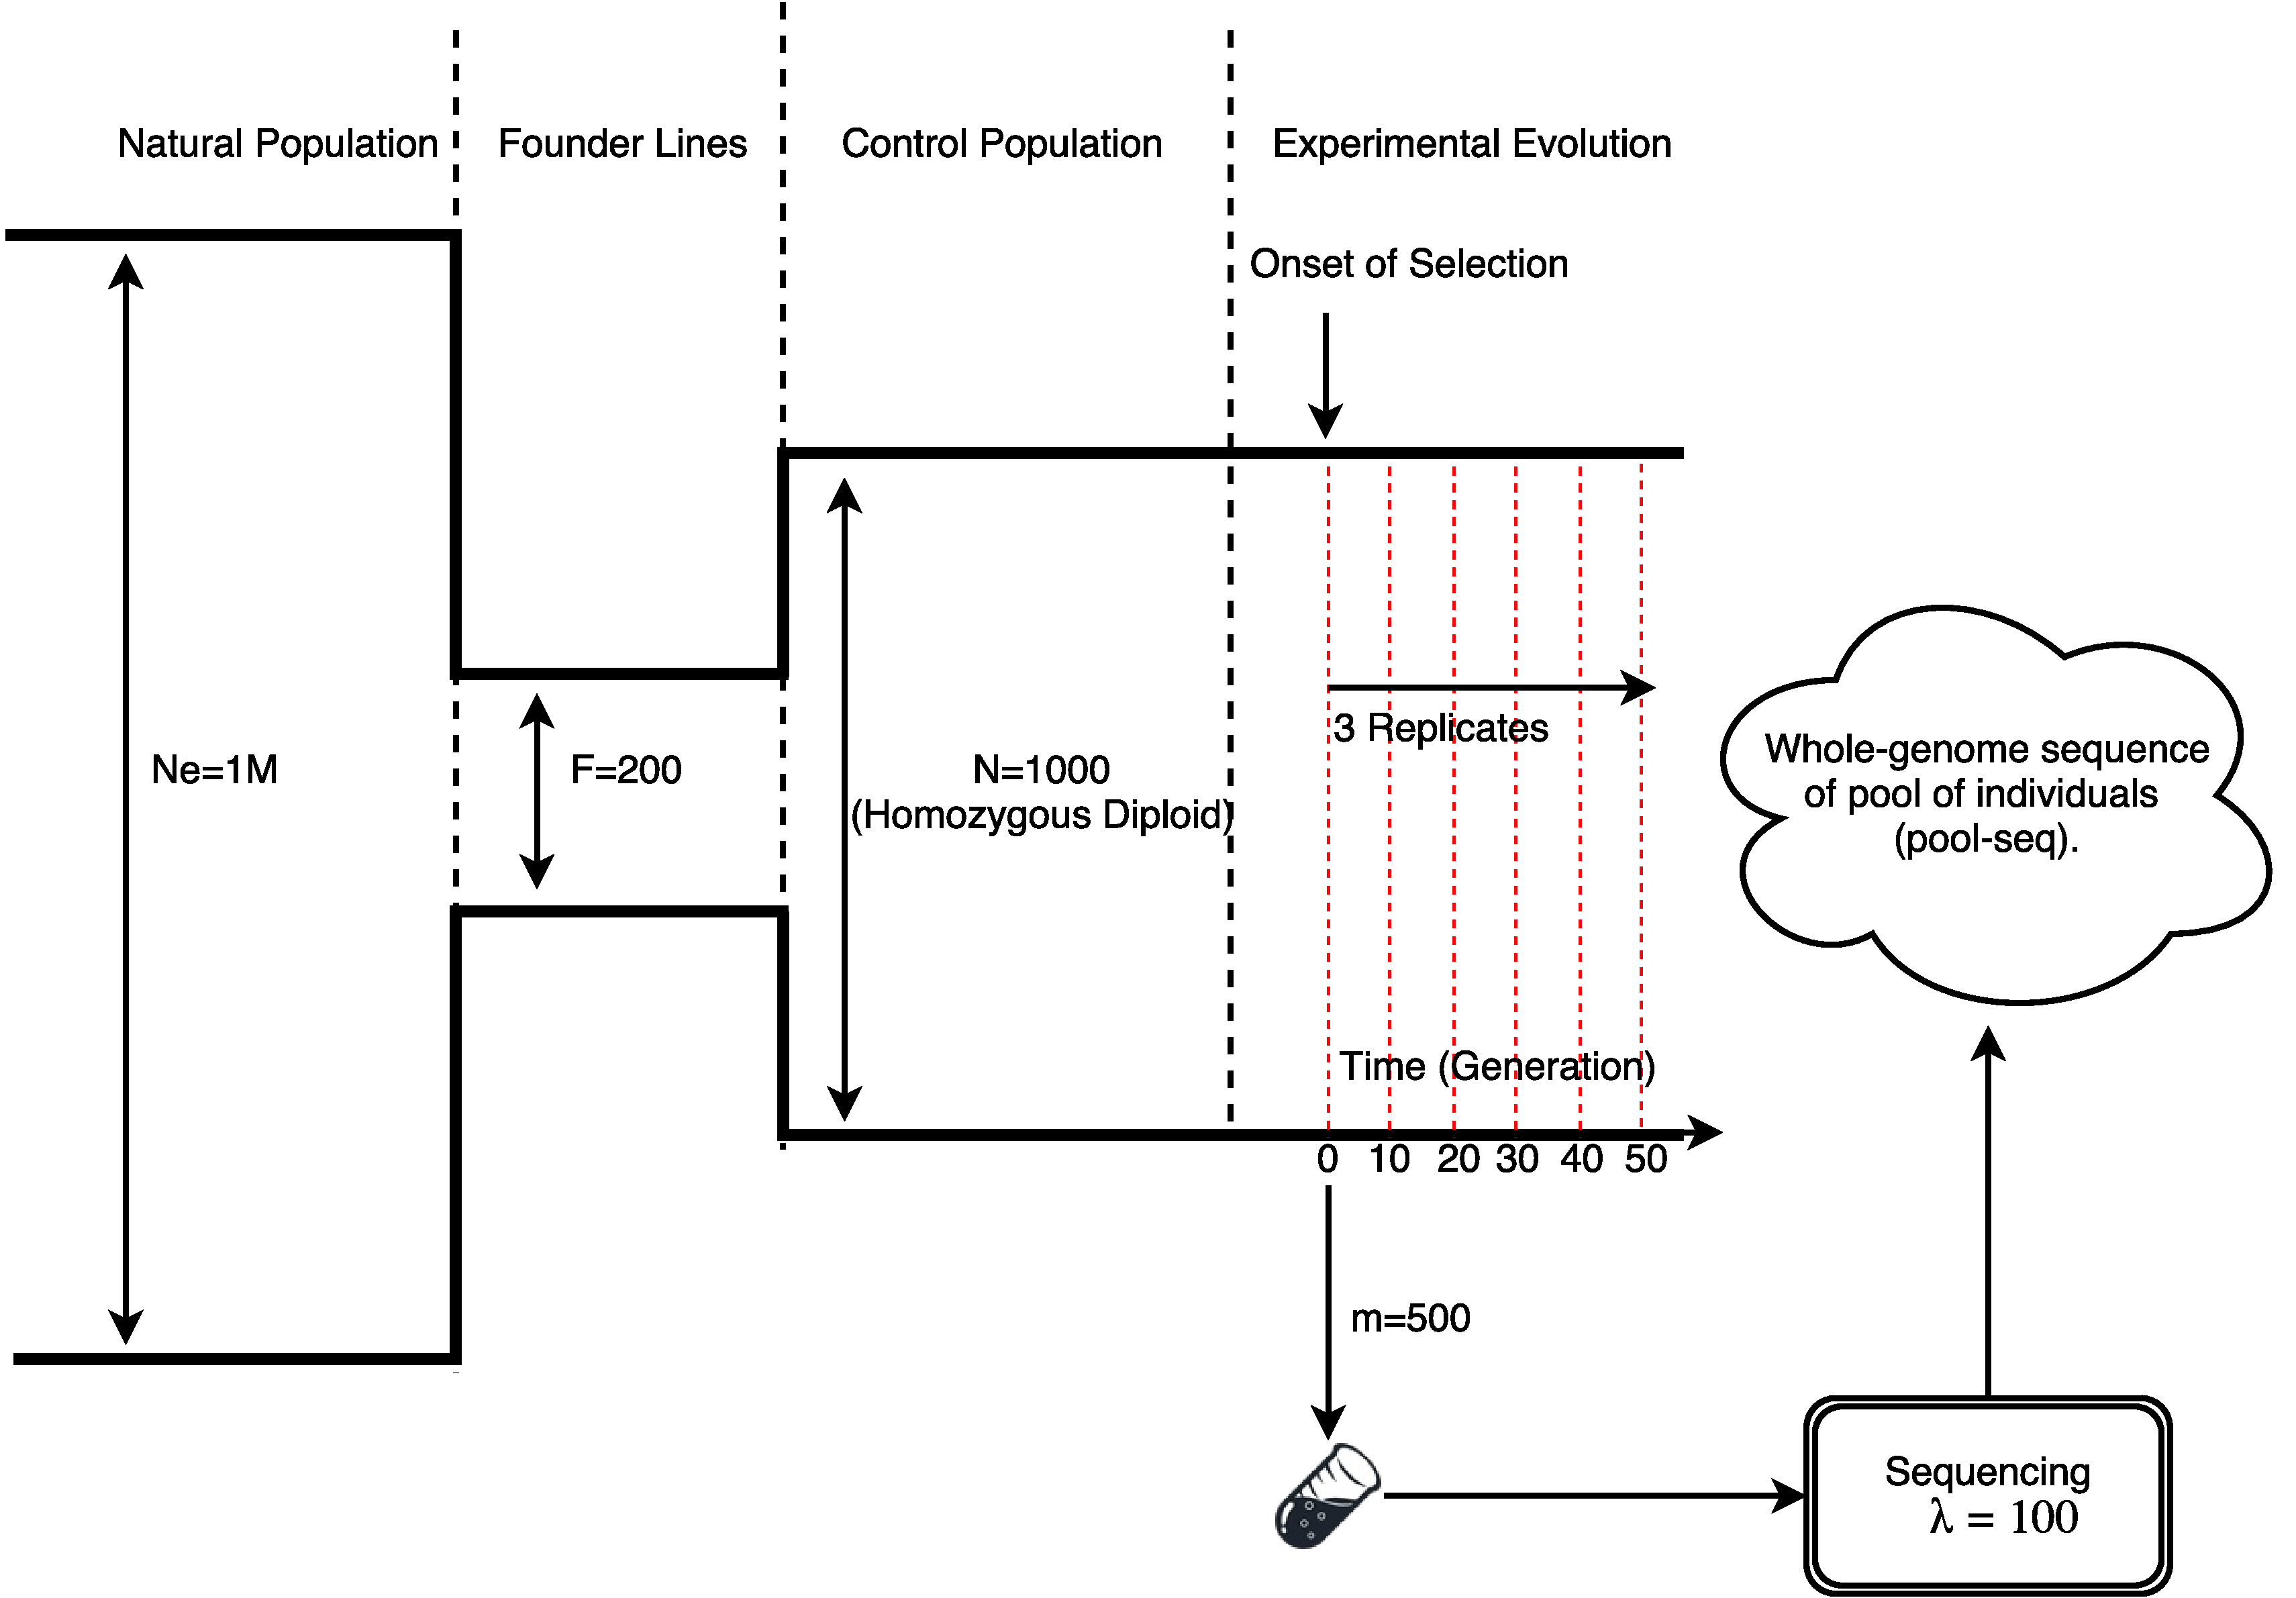
\includegraphics[trim={18in 0.0in 0.0in 
			0in},clip,width=0.8\textwidth]{../figures/ExperimentalEvolution}
	\end{figure}
\end{frame}

\begin{frame}{Whole-Genome Whole-Population Sequencing}
	\begin{itemize}
		\item Pooled-Sequencing 
		\begin{figure}
			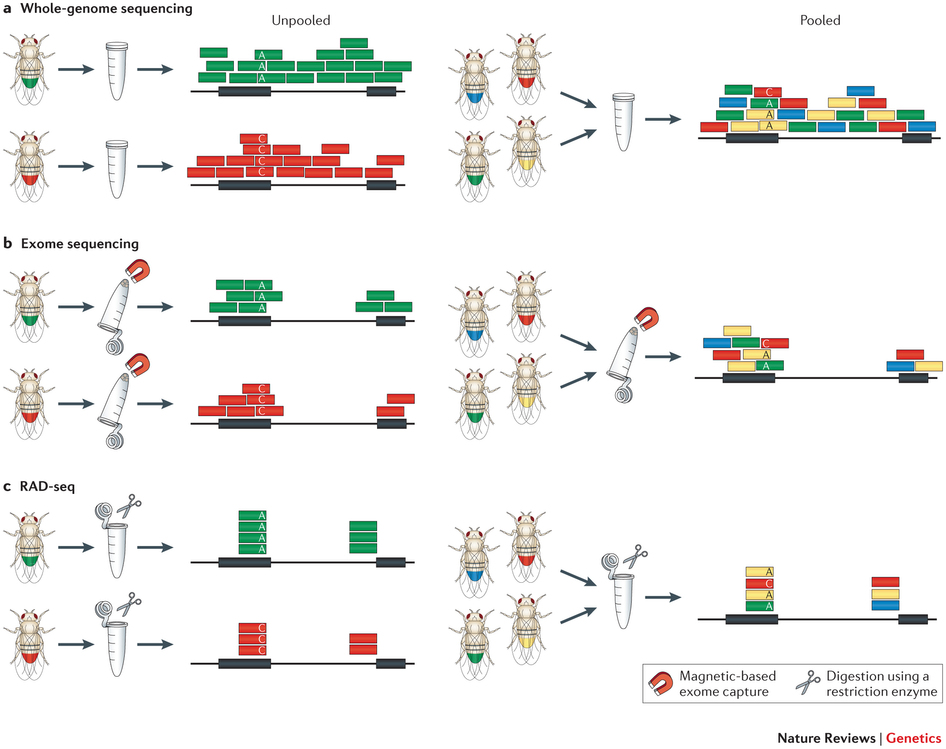
\includegraphics[trim={.05in 7.5in 0.0in 
				0in},clip,width=0.9\textwidth]{../figures/pool-seq}\\
			\tiny{Nature Reviews Genetics 15, 749-763 (2014)}
		\end{figure}
		\pause
			\item Implication: only population allele frequency can be computed.
	\end{itemize}	
\end{frame}

\begin{frame}{Dynamic of population allele frequency }
	under different \emphr{initial conditions} and \emph{selection strengths} 
	frequency 
	change differently
	\begin{figure}
		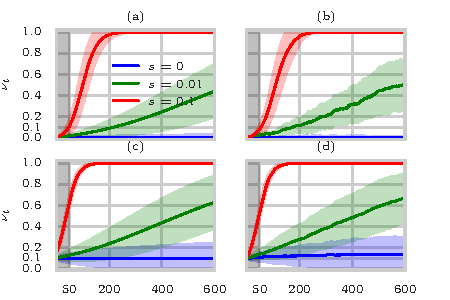
\includegraphics[trim={10in 0.0in 0.0in 
			0in},clip,width=0.7\textwidth]{../figures/AF}
	\end{figure}
\end{frame}


\begin{frame}{ Simplified Model (I)}
	\begin{itemize}
		\item  Suppose we have sequenced a whole (diploid, size=$N$) 
		population \emphr{every 
		generation} (eg, for 6 generations) and \emphr{exact allele 
		frequency} are given.
	\pause
		\item A discrete-time discrete-state model, Markov chain, can 
		generate such a data.
		\begin{figure}
			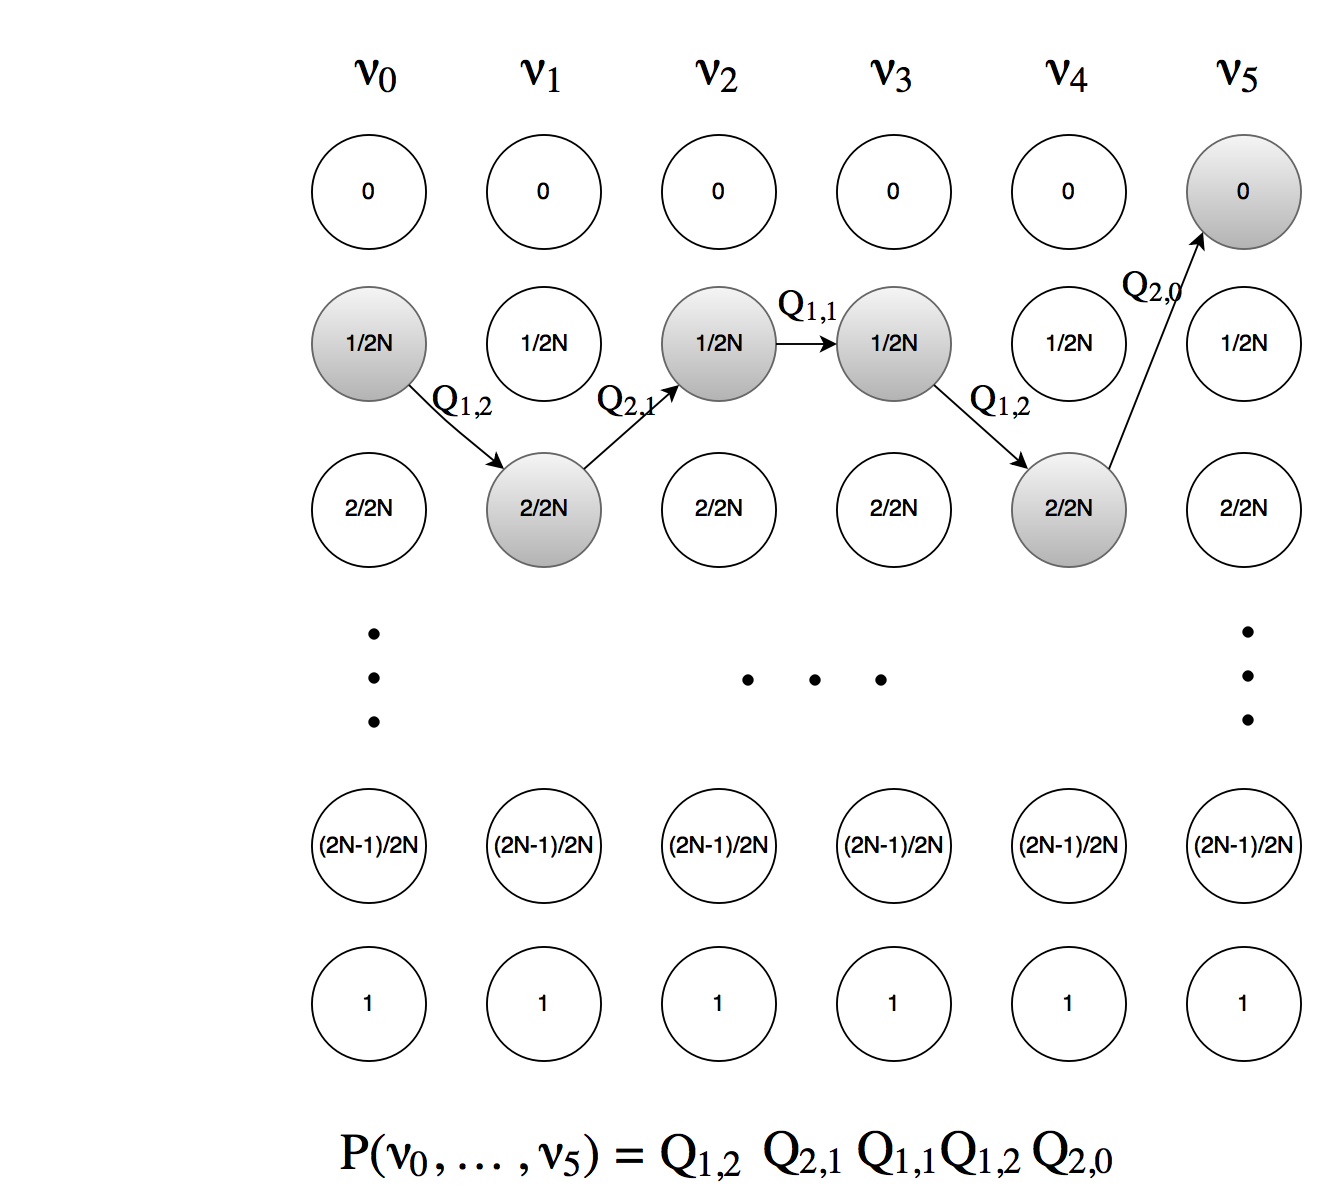
\includegraphics[trim={.05in 0in 0.0in 
				0.5in},clip,width=0.5\textwidth]{../figures/markoveg}
		\end{figure}
	\end{itemize}
\end{frame}

\begin{frame}{ Simplified Model (II)}
	\begin{itemize}
		\item  Where $Q_{i,j}(s,h)$ is the probability of going from frequency 
		$i/(2N)$ to $j/(2N)$ when selection strength is $s$ and over dominance 
		is $h$.
		\pause
		\item Likelihood of parameter can be easily computed
		\beqq
		\Lc(s,h| \{\nu_0,\ldots,\nu_5\}) = \pr(\{\nu_0,\ldots,\nu_5\}| Q(s,h) )
		\eeqq
		\pause
		\item perform maximum likelihood to find $\hat{s}$, $\hat{h}$.
		\pause
		\item compute likelihood ratio, $M$ statistic for each SNP:
		\beqq
		M&=\frac{\text{likelihood of data as if being under 
		selection with } \hat{s},\hat{h}}{l\text{ikelihood 
		of data as if being neutral}}\\
		&=\frac{	\Lc(\hat{s},\hat{h}| \{\nu_0,\ldots,\nu_5\})}{	\Lc(0,0| 
		\{\nu_0,\ldots,\nu_5\})}
		\eeqq
	\end{itemize}
\end{frame}


\begin{frame}{ Model (complete)}
	\begin{itemize}
		\item  In reality, population is sequenced after some ($\tau$) 
		generations.\\
		\emphr{solution: use  $Q^\tau$ in computing likelihoods.}
		\pause
		\item Allele frequencies are unknown, and depth of each variant can be 
		different.\\
		\emphr{solution: extend Markov chain to an HMM by specifying 
		emission probabilities }
	\beqq%	\pr(\text{derived allele read count}|\text{depth},\nu)=\pr(c|d,\nu)\\
	d &\sim \text{Poisson}(\text{Coverage})\\	
	c &\sim \text{Bionomial}(N=d, \theta=\nu)	
	\eeqq
	\pause
	\item everything the is the same, except we need to use \emphr{forward 
	algorithm} to compute likelihood of a sequence of reads.
\pause
	\item Similarly, 
	\beqq
	H&=\frac{\text{likelihood of read-count data as if being under 
			selection }}{l\text{ikelihood 
			of read-count data as if being neutral}}
	\eeqq
	\end{itemize}
\end{frame}

\begin{frame}{Composite Likelihood for a Region (I)}
	\begin{itemize}
		\item So far we developed log-odds ratio statistics $M$ (frequency 
		data) and $H$ (read count data) \emphr{for each variant}.
		\pause
		\item  For a small region with $L$ variants we can simply take the max 
		score in the region, which is prone to \emphr{false positives}.
		\pause
		\item We know that variants are \emphr{correlated}
		\begin{figure}
			\includegraphics[trim={.05in 0in 0.0in 
				0in},clip,width=0.5\textwidth]{../figures/{ld.eg}.png}\\
			\tiny{Crit Care. 2014 Jun 20;18(3):R127}
		\end{figure}
	\end{itemize}
\end{frame}

\begin{frame}{Composite Likelihood for a Region (II)}
	\begin{itemize}
		\item Computing joint likelihoods of SNPs is \emphr{infeasible} 
		(haplotypes are 
		required) and \emphr{intractable} (requires estimating covariance).
		\pause
		\item A heuristic is to compute composite (aka, pseudo) likelihood of  
		the 
		region $L$ to reduce false-positives
		\beqq
		\Hc = \frac{1}{|L|}\sum_{\ell \in L}H_\ell
		\eeqq
	\end{itemize}
\end{frame}


\begin{frame}{ Performance in Detecting Regions under Selection}
Each point represent power  (TPR when FPR$\le$0.05) of detection in 1000 
simulations (500 neutral, 500 selection) of a 50Kbp window, for different 
coverages.
		\begin{figure}
			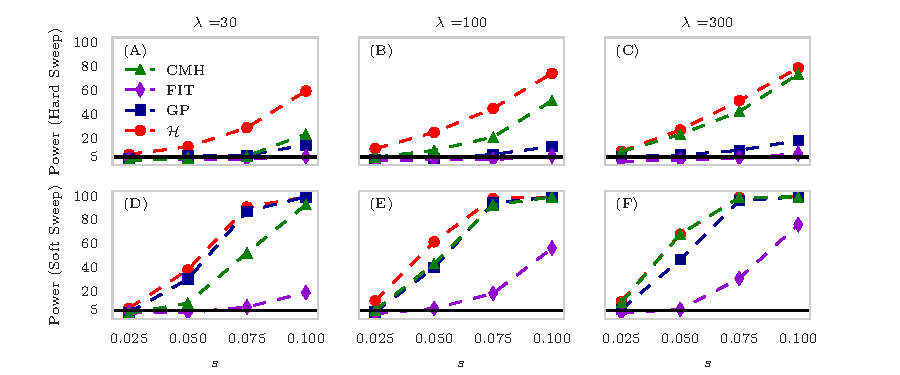
\includegraphics[trim={.05in .0in 0.0in 
				0in},clip,width=\textwidth]{../figures/power.pdf}
		\end{figure}
\end{frame}

\begin{frame}{ Detecting regions under selection: Observations}
\begin{enumerate}[(i)]
	\item Provides better and much robust performances to change of coverage.
	\pause
	\item It can detect well even when coverage is low, i.e., favored allele 
	frequency (1/200 in hard 
	sweep) is below accuracy of sequencing (1/30).
	\pause
	\item Run time is better or comparable with others.
	\begin{figure}
		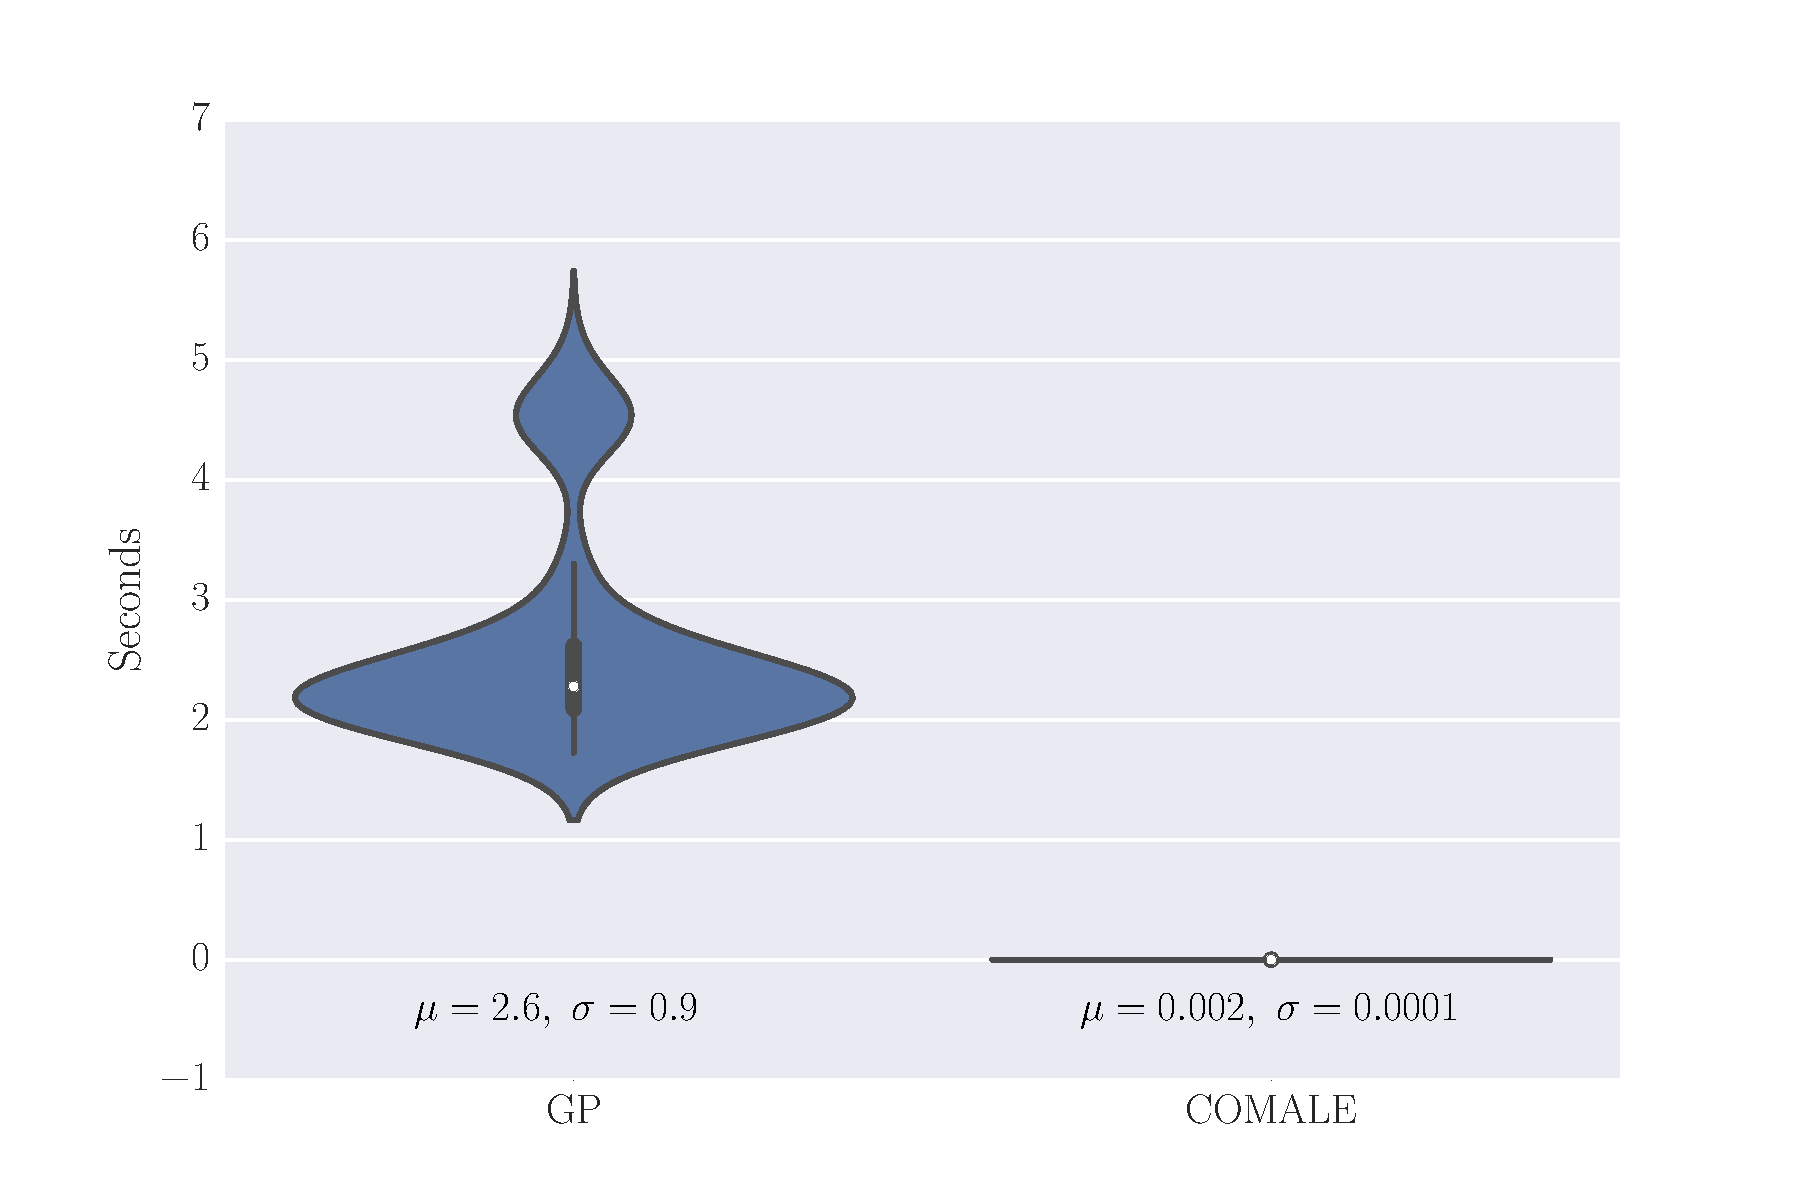
\includegraphics[trim={.0in .0in 0.0in 
			0in},clip,width=0.5\textwidth]{../figures/runTime.pdf}
	\end{figure}
\end{enumerate}
\end{frame}


\begin{frame}{ Localizing favored allele}
Each curve depicts cumulative distribution of the rank  of favored allele among 
($\approx$ 1150) variants, in 500 simulations.

	\begin{figure}
		\includegraphics[trim={.05in .0in 0.0in 
			0in},clip,width=\textwidth]{../figures/{rank100.0}.pdf}
	\end{figure}
\end{frame}


\begin{frame}{ Estimating parameters (I)}
Our model estimates strength of selection $s$ and overdominance 
		$h$ parameter for each variant.
	\begin{figure}
			\includegraphics[trim={.0in .0in 0.0in 
				0in},clip,width=0.5\textwidth]{../figures/{dominance}.pdf}
	\end{figure}
		\begin{itemize}
			\item $h=0$ : recessive adaptive allele
			\item 				$h=0.5$ : directional selection
			\item $h=1$:	dominant adaptive allele
			\item 				$h>1$ :overdominance
		\end{itemize}
\end{frame}


\begin{frame}{ Estimating parameters (II)}
	Distribution of bias of parameters in 500 simulations.
	\begin{figure}
		\includegraphics[trim={.05in .0in 0.0in 
			0in},clip,width=0.6\textwidth]{../figures/{bias.100}.pdf}
	\end{figure}
\end{frame}

\begin{frame}{ Analysis of real data}
\begin{itemize}
	\item A population of \dmel is evolved for 59 generations, under 
	alternative hot and cold temperatures.
	\pause
	\item Coverage is different at generations and samples are not synchronized.
	\pause
	\item Genome scan for sliding window size=50Kbp,  steps=10Kbp
		\begin{figure}
			\includegraphics[trim={.05in .0in 0.0in 
				0in},clip,width=0.8\textwidth]{../figures/{manhattan.min500snp}.pdf}
		\end{figure}		
\end{itemize}
\end{frame}




\begin{frame}{ Discussion}
	\begin{itemize}
		\item An efficient method for analyzing \emphr{ full time-series 
		read-count data} is proposed.
		\pause
		\item By computing composite likelihood $\Hc$ statistic is more robust 
		to false positives.	
		\pause 
		\item When initial frequency of the favored allele is low, stronger 
		selection helps detecting selection but makes locating favored allele a 
		harder task.
		\item Next step is to apply to new dataset with a well defined 
		phenotype, e.g. response to hypoxia.
	\end{itemize}
\end{frame}

\begin{frame}{\ }
	\vspace{1	in}
	\begin{center}
		\huge{Thanks!}\\
	\end{center}
	
\end{frame}
\end{document}